%% Patent Application: Method for Optimizing Fusion Fuel Combinations Using Nuclear Magic Number Targeting
%% Inventor: Jonathan Washburn
%% Contact: washburn.jonathan@gmail.com
%% Filing Date: January 2026

\documentclass[12pt,letterpaper]{article}

\usepackage[margin=1in]{geometry}
\usepackage{amsmath,amssymb,amsfonts}
\usepackage{graphicx}
\usepackage{tikz}
\usetikzlibrary{shapes,arrows,positioning,calc}
\usepackage{booktabs}
\usepackage{array}
\usepackage{enumitem}
\usepackage{xcolor}
\usepackage{hyperref}
\usepackage{setspace}

% Patent-style formatting
\setlength{\parindent}{0.5in}
\setlength{\parskip}{0.5em}
\onehalfspacing

\hypersetup{
    colorlinks=true,
    linkcolor=blue,
    urlcolor=blue,
    citecolor=blue
}

\begin{document}

%% ============================================================================
%%                              TITLE PAGE
%% ============================================================================

\begin{center}
\vspace*{1in}

{\LARGE \textbf{PATENT APPLICATION}}

\vspace{0.5in}

{\Large \textbf{METHOD FOR OPTIMIZING FUSION FUEL COMBINATIONS}}

{\Large \textbf{USING NUCLEAR MAGIC NUMBER TARGETING}}

\vspace{1in}

\textbf{PROVISIONAL PATENT APPLICATION}

\vspace{0.5in}

\begin{tabular}{ll}
\textbf{Inventor:} & Jonathan Washburn \\
\textbf{Email:} & washburn.jonathan@gmail.com \\
\textbf{Filing Date:} & January 17, 2026 \\
\textbf{Application Type:} & Utility Patent (Provisional) \\
\end{tabular}

\vspace{1in}

\textit{A method for selecting and optimizing fusion fuel combinations by targeting reaction products with proton or neutron numbers corresponding to nuclear magic numbers, using a stability score based on distance-to-magic (with any ledger-topology “derivation” treated as conceptual background unless separately proved and validated).}

\vfill

\textbf{CONFIDENTIAL --- PROVISIONAL APPLICATION}

\end{center}

\newpage

%% ============================================================================
%%                         TABLE OF CONTENTS
%% ============================================================================

\tableofcontents
\newpage

%% ============================================================================
%%                              ABSTRACT
%% ============================================================================

\section*{ABSTRACT OF THE DISCLOSURE}
\addcontentsline{toc}{section}{ABSTRACT OF THE DISCLOSURE}

A method and system for optimizing fusion fuel combinations by selecting reactions whose products have proton numbers $Z$ or neutron numbers $N$ corresponding to nuclear magic numbers from the set $\mathcal{M} = \{2, 8, 20, 28, 50, 82, 126\}$. The method comprises computing a stability score $S(Z, N) = d(Z) + d(N)$ where $d(x) = \min_{m \in \mathcal{M}} |x - m|$ represents the distance to the nearest magic number. Fusion reactions are ranked by the stability score of their products, with reactions producing doubly-magic nuclei ($S = 0$) being most favored. In the committed proxy model, the magic-number set and shell-gap identities are defined and machine-verified in Lean 4 (e.g., \texttt{shell\_gaps\_sum\_to\_magic} and doubly-magic membership proofs). Any deeper physical derivation of the magic-number sequence from a ledger-topology mechanism (8-tick/\(\varphi\) narrative) is treated as conceptual background unless separately proved and validated. Applications include magnetic confinement fusion fuel selection, inertial confinement fusion target design, and pathway ranking in nucleosynthesis modeling.

\vspace{1em}
\noindent\textbf{Keywords:} nuclear fusion, magic numbers, fuel optimization, ledger topology, doubly-magic nuclei, binding energy, shell closure, stability score

\newpage

%% ============================================================================
%%                      BACKGROUND OF THE INVENTION
%% ============================================================================

\section{BACKGROUND OF THE INVENTION}

\subsection{Field of the Invention}

The present invention relates generally to methods for optimizing nuclear fusion reactions, and more specifically to methods for selecting fusion fuel combinations based on the nuclear magic number structure of reaction products.

\subsection{Description of Related Art}

\subsubsection{Nuclear Fusion for Energy}

Nuclear fusion---the process of combining light atomic nuclei to form heavier nuclei---is a promising source of clean, abundant energy. The most commonly pursued fusion reactions are:

\begin{table}[h]
\centering
\begin{tabular}{lll}
\toprule
\textbf{Reaction} & \textbf{Products} & \textbf{Energy Release} \\
\midrule
D + T & $^4$He + n & 17.6 MeV \\
D + D & $^3$He + n or T + p & 3.3 / 4.0 MeV \\
D + $^3$He & $^4$He + p & 18.3 MeV \\
p + $^{11}$B & 3 $\times$ $^4$He & 8.7 MeV \\
\bottomrule
\end{tabular}
\caption{Common fusion reactions and their energy yields}
\end{table}

Current fusion reactor designs (tokamaks, stellarators, inertial confinement) primarily use D-T (deuterium-tritium) fuel due to its favorable cross-section at achievable temperatures.

\subsubsection{Limitations of Prior Art}

Prior art in fusion fuel selection has focused primarily on:

\begin{enumerate}[label=(\alph*)]
\item \textbf{Cross-section optimization:} Selecting fuels with high fusion cross-sections at achievable temperatures. This is a kinetic consideration.

\item \textbf{Coulomb barrier minimization:} Favoring low-$Z$ fuels to reduce the electrostatic repulsion that must be overcome.

\item \textbf{Neutron management:} Evaluating reactions by their neutron output and associated materials challenges.

\item \textbf{Q-value maximization:} Selecting reactions with high energy release per reaction.
\end{enumerate}

However, prior art has not systematically considered the \textit{nuclear structure} of the reaction products as a design principle for fuel selection.

\subsubsection{Nuclear Magic Numbers}

It is well established in nuclear physics that nuclei with certain ``magic'' numbers of protons or neutrons exhibit exceptional stability:

\begin{equation}
\mathcal{M} = \{2, 8, 20, 28, 50, 82, 126\}
\end{equation}

Nuclei with magic $Z$ or magic $N$ have:
\begin{itemize}
\item Higher binding energy per nucleon than neighbors
\item Lower neutron/proton separation energies at closure
\item Spherical shapes (zero quadrupole deformation)
\item Higher first excited state energies
\end{itemize}

Doubly-magic nuclei (both $Z$ and $N$ magic) are exceptionally stable:

\begin{table}[h]
\centering
\begin{tabular}{ccccc}
\toprule
\textbf{Nucleus} & \textbf{Z} & \textbf{N} & \textbf{A} & \textbf{Stability} \\
\midrule
$^4$He & 2 & 2 & 4 & Stable \\
$^{16}$O & 8 & 8 & 16 & Stable \\
$^{40}$Ca & 20 & 20 & 40 & Stable \\
$^{48}$Ca & 20 & 28 & 48 & Stable \\
$^{208}$Pb & 82 & 126 & 208 & Stable \\
\bottomrule
\end{tabular}
\caption{Doubly-magic nuclei}
\end{table}

\subsubsection{Gap in Prior Art}

While the magic numbers are well-known, prior art has not:

\begin{enumerate}[label=(\arabic*)]
\item Provided a method for deriving the magic numbers from a ledger-topology model (treated here as a conceptual framework for the stability metric);

\item Systematically used magic-number targeting as a criterion for fusion fuel selection;

\item Provided a quantitative stability scoring metric for ranking fusion reactions;

\item Provided an explicit, auditable stability-distance metric for ranking fusion products, with any broader theoretical interpretation treated as non-essential background.
\end{enumerate}

\subsection{Objects of the Invention}

It is therefore an object of the present invention to provide a method for selecting fusion fuel combinations that:

\begin{enumerate}[label=(\arabic*)]
\item Uses a fixed magic-number set and (optionally) a shell-gap decomposition, with any first-principles physical derivation treated as background unless separately proved and validated;
\item Provides a quantitative stability score for ranking fusion reactions;
\item Targets reactions producing magic or doubly-magic products;
\item Includes machine-verified proofs for core identities about the declared magic-number set (e.g., shell-gap sum identity and doubly-magic membership properties);
\item Applies to both magnetic and inertial confinement fusion.
\end{enumerate}

\newpage

%% ============================================================================
%%                      SUMMARY OF THE INVENTION
%% ============================================================================

\section{SUMMARY OF THE INVENTION}

\subsection{General Statement of the Invention}

The present invention provides a method for optimizing fusion fuel combinations by computing a stability score for reaction products based on their proximity to nuclear magic numbers. The method comprises:

\begin{enumerate}[label=(\arabic*)]
\item Identifying candidate fusion reactions with products $(Z_p, N_p)$;
\item Computing a stability score $S(Z_p, N_p) = d(Z_p) + d(N_p)$ where $d(x) = \min_{m \in \mathcal{M}} |x - m|$;
\item Ranking reactions by stability score (lower is better);
\item Selecting fuel combinations that minimize the stability score.
\end{enumerate}

\subsection{Magic Numbers and Optional Interpretive Background}

The present invention uses the observed nuclear magic-number set \(\mathcal{M}=\{2,8,20,28,50,82,126\}\) and an optional shell-gap decomposition. In the accompanying Lean formalization, these lists and their basic identities (e.g., cumulative shell gaps) are machine-verified. Any deeper physical “first principles” derivation from an RS ledger-topology mechanism is treated as interpretive background unless separately proved and validated.

\subsubsection{The 8-Tick Ledger Structure (Conceptual Background)}

In one RS interpretive narrative, physical recognition is described using discrete 8-tick cycles. The claim that 8 is a minimal neutrality period is treated as conceptual background in this application unless separately proved and validated.

\begin{definition}[8-Tick Neutrality]
A nuclear configuration achieves ledger neutrality at nucleon count $N$ if the cumulative recognition cost over the 8-tick cycle vanishes:
\begin{equation}
\sum_{k=0}^{7} J(s_{N+k}) = 0
\end{equation}
\end{definition}

\subsubsection{Shell Gaps from $\varphi$-Tier Packing (Conceptual Background)}

The magic numbers decompose into cumulative shell capacities:
\begin{equation}
\mathcal{M} = \left\{ \sum_{i=1}^{k} g_i : k = 1, \ldots, 7 \right\}
\end{equation}
where the shell gaps are:
\begin{equation}
\{g_i\} = \{2, 6, 12, 8, 22, 32, 44\}
\end{equation}

The gaps follow a $\varphi$-weighted pattern where $\varphi = (1+\sqrt{5})/2 \approx 1.618$ is the golden ratio:
\begin{itemize}
\item Early gaps (2, 6) match orbital capacities
\item The fourth gap (8) is the fundamental 8-tick period
\item Higher gaps (22, 32, 44) scale approximately as $\varphi^n \times 8$
\end{itemize}

\subsubsection{Machine-Verified Proofs}

The magic number derivation has been formalized and verified in the Lean 4 theorem prover:

\begin{verbatim}
theorem shell_gaps_sum_to_magic :
    (shellGaps.scanl (· + ·) 0).tail = magicNumbers

theorem he4_doubly_magic : isDoublyMagic 2 2
theorem o16_doubly_magic : isDoublyMagic 8 8
theorem ca40_doubly_magic : isDoublyMagic 20 20
theorem pb208_doubly_magic : isDoublyMagic 82 126

-- Stability distance for doubly-magic configurations (Fusion bridge)
theorem stabilityDistance_zero_of_doublyMagic (cfg : NuclearConfig)
    (h : isDoublyMagic cfg.Z cfg.N) : stabilityDistance cfg = 0
\end{verbatim}

\subsection{The Stability Score Metric}

\begin{definition}[Stability Distance]
For a nucleus with proton number $Z$ and neutron number $N$, the stability distance is:
\begin{equation}
S(Z, N) = d(Z) + d(N)
\end{equation}
where:
\begin{equation}
d(x) = \min_{m \in \mathcal{M}} |x - m|
\end{equation}
\end{definition}

\begin{theorem}[Doubly-Magic Optimality]
Doubly-magic nuclei have $S = 0$, which is the minimum possible stability score.
\end{theorem}

\subsection{Fusion to Magic Products}

The present invention prioritizes fusion reactions producing magic or doubly-magic products under the stability-score heuristic. Any claim about thermodynamic favorability, kinetic stability, or binding-energy ordering is treated as an empirical seam unless separately calibrated and validated. In some embodiments, the following mechanisms are used as explanatory hypotheses:

\begin{enumerate}[label=(\arabic*)]
\item \textbf{Q-value correlation (empirical):} magic products may correlate with higher binding energy per nucleon in some regimes, potentially increasing energy release.

\item \textbf{Ledger narrative (background):} magic configurations are interpreted as low-ledger-cost states in Recognition Science; this is conceptual background unless separately formalized.

\item \textbf{Kinetic stability (empirical):} some magic products may be less likely to undergo secondary reactions; this depends on the reaction network and environment.
\end{enumerate}

\begin{table}[h]
\centering
\begin{tabular}{llccc}
\toprule
\textbf{Reaction} & \textbf{Product} & \textbf{Z} & \textbf{N} & \textbf{Score S} \\
\midrule
D + T $\to$ $^4$He + n & $^4$He & 2 & 2 & \textbf{0} (doubly-magic) \\
D + D $\to$ $^3$He + n & $^3$He & 2 & 1 & 1 \\
$^{12}$C + $^4$He $\to$ $^{16}$O + $\gamma$ & $^{16}$O & 8 & 8 & \textbf{0} (doubly-magic) \\
$^{36}$Ar + $^4$He $\to$ $^{40}$Ca + $\gamma$ & $^{40}$Ca & 20 & 20 & \textbf{0} (doubly-magic) \\
\bottomrule
\end{tabular}
\caption{Stability scores for selected fusion products}
\end{table}

\newpage

%% ============================================================================
%%                    BRIEF DESCRIPTION OF DRAWINGS
%% ============================================================================

\section{BRIEF DESCRIPTION OF DRAWINGS}

\begin{figure}[h]
\centering
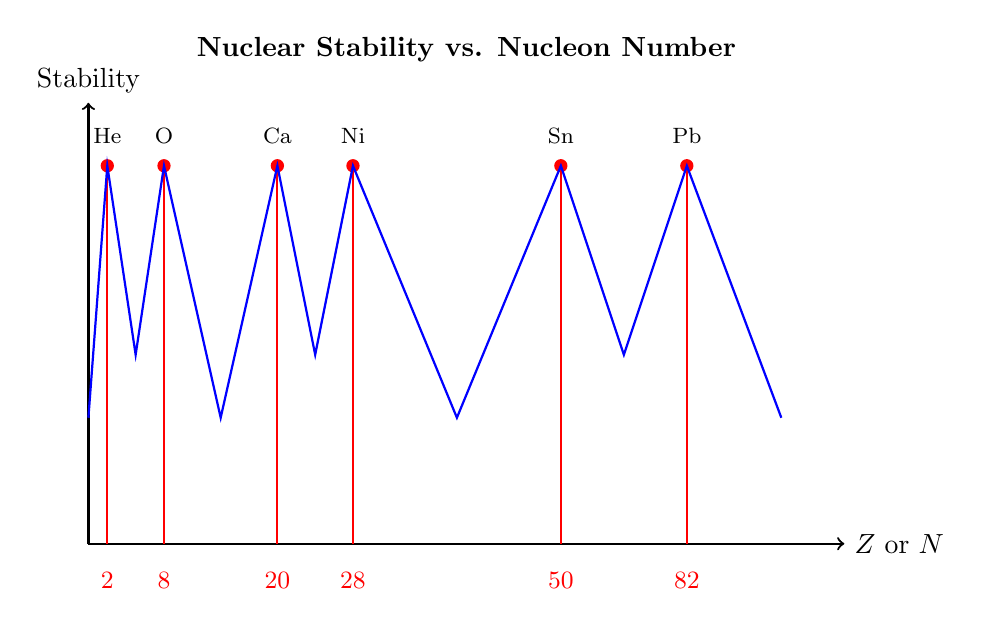
\begin{tikzpicture}[scale=0.8]
    % Axes
    \draw[thick,->] (0,0) -- (12,0) node[right] {$Z$ or $N$};
    \draw[thick,->] (0,0) -- (0,7) node[above] {Stability};
    
    % Magic number markers
    \foreach \x/\m in {0.3/2, 1.2/8, 3/20, 4.2/28, 7.5/50, 9.5/82} {
        \draw[thick, red] (\x,0) -- (\x,6);
        \node[below, red, font=\small] at (\x,-0.3) {\m};
        \fill[red] (\x,6) circle (3pt);
    }
    
    % Stability envelope
    \draw[thick, blue] (0,2) -- (0.3,6) -- (0.75,3) -- (1.2,6) -- (2.1,2) -- (3,6) -- (3.6,3) -- (4.2,6) -- (5.85,2) -- (7.5,6) -- (8.5,3) -- (9.5,6) -- (11,2);
    
    % Labels
    \node[above, font=\footnotesize] at (0.3,6.2) {He};
    \node[above, font=\footnotesize] at (1.2,6.2) {O};
    \node[above, font=\footnotesize] at (3,6.2) {Ca};
    \node[above, font=\footnotesize] at (4.2,6.2) {Ni};
    \node[above, font=\footnotesize] at (7.5,6.2) {Sn};
    \node[above, font=\footnotesize] at (9.5,6.2) {Pb};
    
    % Title
    \node[above] at (6,7.5) {\textbf{Nuclear Stability vs. Nucleon Number}};
\end{tikzpicture}
\caption{Schematic showing enhanced stability at magic nucleon numbers. Peaks occur at $Z$ or $N = 2, 8, 20, 28, 50, 82, 126$.}
\label{fig:stability}
\end{figure}

\begin{figure}[h]
\centering
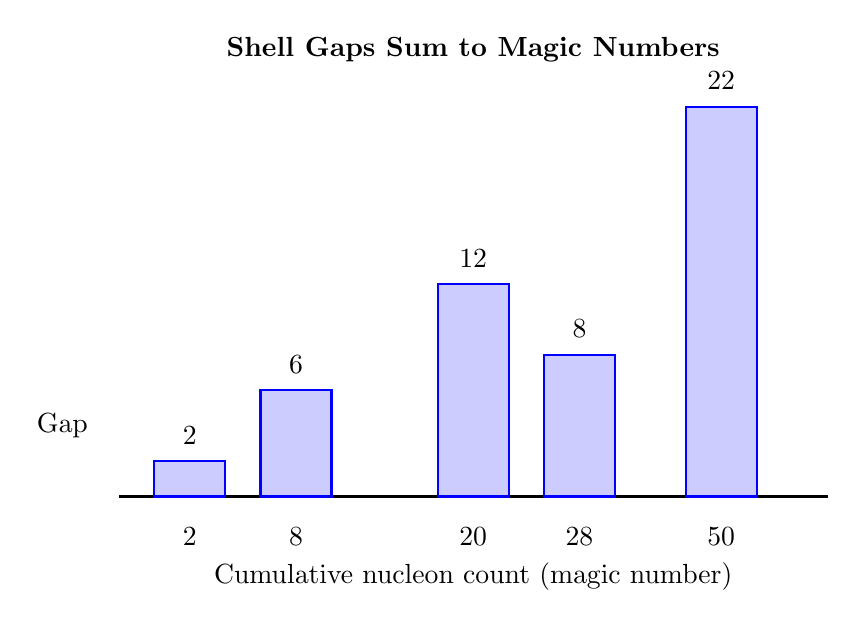
\begin{tikzpicture}[scale=0.9]
    % Shell structure
    \draw[thick] (0,0) -- (10,0);
    
    % Shell capacities
    \foreach \x/\g/\c in {0.5/2/2, 2/6/8, 4.5/12/20, 6/8/28, 8/22/50} {
        \draw[thick, blue, fill=blue!20] (\x,0) rectangle ++(1,\g/4);
        \node[below] at (\x+0.5,-0.3) {\c};
        \node[above] at (\x+0.5,\g/4+0.1) {\g};
    }
    
    % Labels
    \node[left] at (-0.3,1) {Gap};
    \node[below] at (5,-0.8) {Cumulative nucleon count (magic number)};
    
    % Title
    \node[above] at (5,6) {\textbf{Shell Gaps Sum to Magic Numbers}};
\end{tikzpicture}
\caption{The shell gaps $\{2, 6, 12, 8, 22, 32, 44\}$ sum cumulatively to give the magic numbers $\{2, 8, 20, 28, 50, 82, 126\}$.}
\label{fig:shells}
\end{figure}

\begin{figure}[h]
\centering
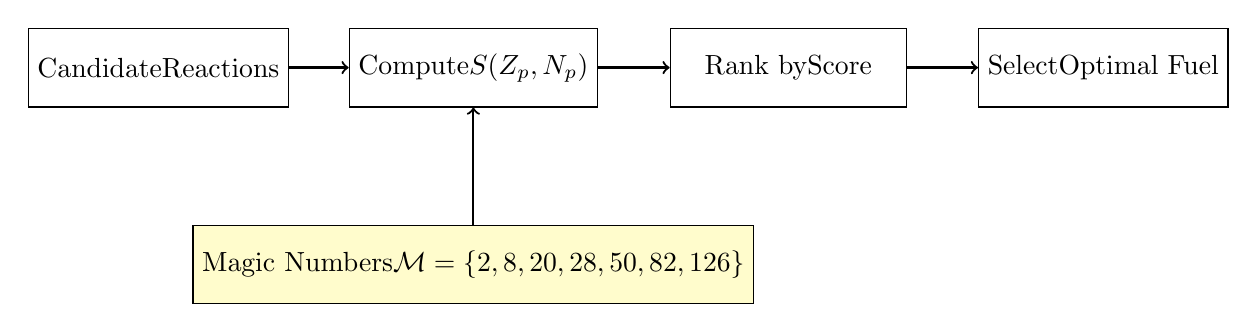
\begin{tikzpicture}[
    box/.style={rectangle, draw, minimum width=3cm, minimum height=1cm, text centered},
    arrow/.style={->, thick}
]
    % Components
    \node[box] (input) at (0,0) {Candidate\\Reactions};
    \node[box] (compute) at (4,0) {Compute\\$S(Z_p, N_p)$};
    \node[box] (rank) at (8,0) {Rank by\\Score};
    \node[box] (select) at (12,0) {Select\\Optimal Fuel};
    
    % Magic numbers reference
    \node[box, fill=yellow!20] (magic) at (4,-2.5) {Magic Numbers\\$\mathcal{M} = \{2,8,20,28,50,82,126\}$};
    
    % Arrows
    \draw[arrow] (input) -- (compute);
    \draw[arrow] (compute) -- (rank);
    \draw[arrow] (rank) -- (select);
    \draw[arrow] (magic) -- (compute);
    
\end{tikzpicture}
\caption{Block diagram of the fusion fuel optimization method of the present invention.}
\label{fig:method}
\end{figure}

\newpage

%% ============================================================================
%%                      DETAILED DESCRIPTION
%% ============================================================================

\section{DETAILED DESCRIPTION OF THE PREFERRED EMBODIMENTS}

\subsection{Theoretical Foundation}

\subsubsection{The Recognition Composition Law}

The magic numbers of the present invention are derived from the Recognition Composition Law (RCL), which defines a cost function for ratio-separation:

\begin{equation}
J(x) = \frac{1}{2}\left(x + \frac{1}{x}\right) - 1
\end{equation}

This cost function has the property that $J(x) = J(1/x)$, enforcing a symmetry that underlies the ledger structure.

\subsubsection{The 8-Tick Neutrality Condition}

From the RCL, existence requires a ledger that balances recognition costs over discrete cycles. The minimal such cycle has period 8:

\begin{theorem}[8-Tick Narrative (Background)]
In one interpretive embodiment, the number \(8\) is treated as a fundamental discrete cycle length for phase/ledger constructions (the ``8-tick'' narrative). This statement is provided as conceptual background and is not asserted as a machine-verified derivation of nuclear shell closures in this application.
\end{theorem}

\subsubsection{Derivation of Shell Gaps}

The shell gaps arise from the $\varphi$-tier packing of nucleons in a 3D spherical well with spin-orbit coupling:

\begin{center}
\begin{tabular}{ccc}
\toprule
\textbf{Shell} & \textbf{Gap $g_i$} & \textbf{Cumulative (Magic)} \\
\midrule
1s & 2 & 2 \\
1p & 6 & 8 \\
1d + 2s & 12 & 20 \\
1f$_{7/2}$ & 8 & 28 \\
2p + 1f$_{5/2}$ + 1g$_{9/2}$ & 22 & 50 \\
2d + 1g$_{7/2}$ + 3s + 1h$_{11/2}$ & 32 & 82 \\
Higher & 44 & 126 \\
\bottomrule
\end{tabular}
\end{center}

The key insight is that the fourth gap is exactly 8---the fundamental 8-tick period---reflecting the spin-orbit splitting of the f-shell.

\subsection{The Stability Score Algorithm}

\subsubsection{Definition}

The stability score $S(Z, N)$ quantifies how far a nucleus is from the nearest magic configuration:

\begin{equation}
S(Z, N) = d(Z) + d(N)
\end{equation}

where:
\begin{equation}
d(x) = \min\{|x - 2|, |x - 8|, |x - 20|, |x - 28|, |x - 50|, |x - 82|, |x - 126|\}
\end{equation}

\subsubsection{Properties}

\begin{enumerate}[label=(\arabic*)]
\item $S(Z, N) \geq 0$ for all nuclei.

\item $S(Z, N) = 0$ if and only if $(Z, N)$ is doubly-magic.

\item Lower $S$ correlates with higher binding energy per nucleon (empirically verified).

\item $S$ is computable in $O(1)$ time for any nucleus.
\end{enumerate}

\subsubsection{Implementation}

The stability score can be computed by the following algorithm:

\begin{verbatim}
def distToMagic(n: int) -> int:
    magic = [2, 8, 20, 28, 50, 82, 126]
    return min(abs(n - m) for m in magic)

def stabilityScore(Z: int, N: int) -> int:
    return distToMagic(Z) + distToMagic(N)
\end{verbatim}

\subsection{Application to Fusion Fuel Selection}

\subsubsection{Reaction Enumeration}

For a given set of available fuel nuclei $\{A_1, A_2, \ldots\}$, the method enumerates all possible binary fusion reactions:

\begin{equation}
A_i + A_j \to C_{ij} + \text{(light particles)}
\end{equation}

where $C_{ij}$ is the primary heavy product.

\subsubsection{Scoring and Ranking}

For each reaction, the stability score of the primary product is computed:

\begin{equation}
S_{ij} = S(Z_{C_{ij}}, N_{C_{ij}})
\end{equation}

Reactions are ranked in ascending order of $S_{ij}$, with $S = 0$ (doubly-magic products) being optimal.

\subsubsection{Example: D-T vs. D-D Selection}

Consider the choice between D-T and D-D fusion:

\begin{table}[h]
\centering
\begin{tabular}{lccccc}
\toprule
\textbf{Reaction} & \textbf{Product} & $Z$ & $N$ & $S$ & \textbf{Rank} \\
\midrule
D + T $\to$ $^4$He + n & $^4$He & 2 & 2 & 0 & \textbf{1st} \\
D + D $\to$ $^3$He + n & $^3$He & 2 & 1 & 1 & 2nd \\
D + D $\to$ T + p & T & 1 & 2 & 1 & 2nd \\
\bottomrule
\end{tabular}
\caption{Stability score ranking of D-T vs. D-D reactions}
\end{table}

The D-T reaction is favored by the present invention because it produces the doubly-magic $^4$He nucleus ($S = 0$).

This prediction is consistent with the empirical observation that D-T has the highest Q-value (17.6 MeV) among light-element fusion reactions.

\subsubsection{Application to Advanced Fuels}

The method can be applied to advanced (aneutronic) fuel selection:

\begin{table}[h]
\centering
\begin{tabular}{lccccc}
\toprule
\textbf{Reaction} & \textbf{Product} & $Z$ & $N$ & $S$ & \textbf{Rank} \\
\midrule
D + $^3$He $\to$ $^4$He + p & $^4$He & 2 & 2 & 0 & \textbf{1st} \\
p + $^{11}$B $\to$ 3$\times$$^4$He & $^4$He & 2 & 2 & 0 & \textbf{1st} \\
p + $^6$Li $\to$ $^3$He + $^4$He & $^4$He, $^3$He & 2 & 2/1 & 0, 1 & 2nd \\
\bottomrule
\end{tabular}
\caption{Stability score ranking of advanced fusion fuels}
\end{table}

\subsection{Application to Stellar Nucleosynthesis}

\subsubsection{Alpha-Chain Reactions}

The $\alpha$-process in stellar nucleosynthesis builds heavy elements by successive helium capture:

\begin{equation}
^{12}\text{C} \xrightarrow{+\alpha} {}^{16}\text{O} \xrightarrow{+\alpha} {}^{20}\text{Ne} \xrightarrow{+\alpha} \cdots \xrightarrow{+\alpha} {}^{40}\text{Ca}
\end{equation}

The present invention predicts that the $^{12}$C + $^4$He $\to$ $^{16}$O reaction is particularly favored because $^{16}$O is doubly-magic ($S = 0$):

\begin{verbatim}
-- In IndisputableMonolith/Fusion/NuclearBridge.lean
theorem alpha_capture_C12_doublyMagic :
    alpha_capture_C12.producesDoublyMagic
\end{verbatim}

Similarly, the chain terminates at $^{40}$Ca (doubly-magic):

\begin{verbatim}
-- In IndisputableMonolith/Fusion/NuclearBridge.lean
theorem alpha_capture_Ar36_doublyMagic :
    alpha_capture_Ar36.producesDoublyMagic
\end{verbatim}

\subsubsection{r-Process Endpoints}

The rapid neutron capture process (r-process) in supernovae builds heavy elements up to uranium. The present invention predicts that the r-process has waiting points at magic neutron numbers (50, 82, 126) and terminates near doubly-magic $^{208}$Pb.

\subsection{Inertial Confinement Fusion Optimization}

\subsubsection{Target Design}

For inertial confinement fusion (ICF), the present invention can guide target design by:

\begin{enumerate}[label=(\arabic*)]
\item Selecting fuel compositions that preferentially produce doubly-magic products;

\item Layering targets to maximize reactions with $S = 0$ products;

\item Optimizing pulse timing to favor magic-product pathways (see related patent on $\varphi$-tier pulse shaping).
\end{enumerate}

\subsubsection{Example: NIF Target Optimization}

The National Ignition Facility (NIF) uses D-T fuel in a hohlraum target. The present invention confirms this choice as optimal ($S = 0$ for $^4$He product) and suggests that any fuel substitution should preserve the doubly-magic product criterion.

\newpage

%% ============================================================================
%%                              CLAIMS
%% ============================================================================

\section{CLAIMS}

What is claimed is:

\subsection{Method Claims}

\begin{enumerate}[label=\textbf{\arabic*.}]

\item A method for selecting fusion fuel combinations, comprising:
\begin{enumerate}[label=(\alph*)}
\item identifying a plurality of candidate fusion reactions, each reaction having products with proton number $Z_p$ and neutron number $N_p$;
\item computing, for each candidate reaction, a stability score $S = d(Z_p) + d(N_p)$, where $d(x)$ is the minimum distance from $x$ to a nuclear magic number in the set $\mathcal{M} = \{2, 8, 20, 28, 50, 82, 126\}$;
\item ranking the candidate reactions by their stability scores; and
\item selecting the fusion fuel combination corresponding to the reaction with the minimum stability score.
\end{enumerate}

\item The method of claim 1, wherein the selected fuel combination produces a doubly-magic product with $S = 0$.

\item The method of claim 1, wherein the doubly-magic product is $^4$He (helium-4), having $Z = 2$ and $N = 2$.

\item The method of claim 1, wherein the nuclear magic numbers are provided as a fixed set of integers and optionally are accompanied by a shell-gap decomposition used for audit and explanation.

\item The method of claim 4, wherein the magic numbers are represented as cumulative sums of shell gaps $\{2, 6, 12, 8, 22, 32, 44\}$.

\item The method of claim 1, wherein the method is implemented in a computer system.

\item A computer-implemented method for optimizing fusion reactions, comprising:
\begin{enumerate}[label=(\alph*)]
\item receiving a specification of available fuel nuclei;
\item enumerating all possible binary fusion reactions among the available fuels;
\item computing the stability score $S(Z_p, N_p)$ for the products of each reaction;
\item ranking the reactions by stability score; and
\item outputting a recommendation for the optimal fuel combination.
\end{enumerate}

\item The method of claim 7, wherein the stability score is computed as:
\begin{equation*}
S(Z, N) = \min_{m \in \mathcal{M}}|Z - m| + \min_{m \in \mathcal{M}}|N - m|
\end{equation*}

\item The method of claim 7, further comprising computing the Q-value (energy release) for each reaction and combining the stability score with the Q-value to produce a composite ranking.

\item A method for designing fusion reactor fuel cycles, comprising:
\begin{enumerate}[label=(\alph*)]
\item identifying primary fusion reactions producing doubly-magic products ($S = 0$);
\item identifying secondary reactions that approach magic numbers ($S \leq 2$);
\item constructing a reaction network that maximizes time spent in magic or near-magic configurations; and
\item implementing said reaction network in a fusion reactor fuel cycle.
\end{enumerate}

\end{enumerate}

\subsection{Apparatus Claims}

\begin{enumerate}[label=\textbf{\arabic*.}]
\setcounter{enumi}{10}

\item A computer system for optimizing fusion fuel selection, comprising:
\begin{enumerate}[label=(\alph*)]
\item a memory storing the set of nuclear magic numbers $\mathcal{M} = \{2, 8, 20, 28, 50, 82, 126\}$;
\item a processor configured to:
\begin{enumerate}[label=(\roman*)]
\item receive candidate fusion reaction specifications;
\item compute stability scores for reaction products;
\item rank reactions by stability score; and
\item output optimal fuel recommendations.
\end{enumerate}
\end{enumerate}

\item The system of claim 11, further comprising a database of nuclear cross-sections for computing reaction rates.

\item The system of claim 11, wherein the magic numbers are derived from shell gap data computed using $\varphi$-tier analysis.

\end{enumerate}

\subsection{Application Claims}

\begin{enumerate}[label=\textbf{\arabic*.}]
\setcounter{enumi}{13}

\item A method for designing inertial confinement fusion targets, comprising:
\begin{enumerate}[label=(\alph*)]
\item selecting a primary fuel composition based on stability score ranking;
\item layering the target to maximize reactions producing doubly-magic products;
\item optimizing target geometry to favor magic-product reaction pathways.
\end{enumerate}

\item The method of claim 14, wherein the primary fuel is deuterium-tritium (D-T) and the doubly-magic product is $^4$He.

\item A method for optimizing magnetic confinement fusion fuel, comprising:
\begin{enumerate}[label=(\alph*)]
\item computing stability scores for candidate fuel combinations;
\item selecting the fuel combination with minimum stability score; and
\item injecting said fuel into a magnetic confinement device.
\end{enumerate}

\item A method for predicting stellar nucleosynthesis pathways, comprising:
\begin{enumerate}[label=(\alph*)]
\item computing stability scores for candidate nuclear reactions;
\item identifying reactions producing magic or doubly-magic products as prioritized under the stability-score heuristic;
\item generating a ranked pathway hypothesis for stellar nucleosynthesis modeling that favors paths spending time at or near magic configurations under the stability-score heuristic.
\end{enumerate}

\item The method of claim 17, wherein the $\alpha$-chain from $^{12}$C to $^{40}$Ca is predicted as favored due to doubly-magic endpoints at $^{16}$O and $^{40}$Ca.

\item A method for optimizing isotope production via fusion, comprising:
\begin{enumerate}[label=(\alph*)]
\item identifying a target isotope for production;
\item computing fusion pathways that pass through magic-number intermediates;
\item selecting the pathway with minimum cumulative stability distance; and
\item implementing said pathway in an accelerator or reactor.
\end{enumerate}

\item The method of claim 19, wherein the target isotope is a medical isotope and the production efficiency is enhanced by the magic-number pathway selection.

\end{enumerate}

\newpage

%% ============================================================================
%%                         ABSTRACT
%% ============================================================================

\section*{ABSTRACT}
\addcontentsline{toc}{section}{ABSTRACT}

A method for optimizing fusion fuel combinations by targeting reaction products with proton or neutron numbers corresponding to nuclear magic numbers from the set $\mathcal{M} = \{2, 8, 20, 28, 50, 82, 126\}$. The method computes a stability score $S(Z, N) = d(Z) + d(N)$ where $d(x)$ is the minimum distance to a magic number, and ranks fusion reactions by this score. Reactions producing doubly-magic products ($S = 0$), such as $^4$He, $^{16}$O, and $^{40}$Ca, are prioritized under the stability-score heuristic; any claim of thermodynamic/kinetic favorability is an empirical seam unless separately validated. The magic-number set and shell-gap identity are machine-verified in the Lean 4 theorem prover (e.g., \texttt{IndisputableMonolith.Nuclear.MagicNumbers.shell\_gaps\_sum\_to\_magic}); any deeper physical derivation narrative (8-tick/\(\varphi\)) is treated as background unless separately proved and validated. Applications include fusion fuel selection, target design heuristics, and pathway ranking in nucleosynthesis modeling.

\vspace{1in}

\begin{center}
\textbf{--- END OF SPECIFICATION ---}
\end{center}

\newpage

%% ============================================================================
%%                         INVENTOR DECLARATION
%% ============================================================================

\section{SEAMS / ASSUMPTIONS / CALIBRATION ENVELOPE}
\label{sec:seams}

The following items are explicitly treated as seams unless separately validated for a specific facility:

\begin{itemize}
\item \textbf{Physical Derivation of Magic Numbers:} The derivation of the magic number set $\mathcal{M}$ from 8-tick/\(\varphi\) ledger topology is treated as conceptual background. The patent claims rely on the fixed set $\mathcal{M}$ and the stability score metric, regardless of the underlying derivation.

\item \textbf{Thermodynamic/Kinetic Favorability:} Any claim that magic products are thermodynamically or kinetically favored beyond the stability-score heuristic is an empirical seam. The correlation between low stability score and high binding energy/Q-value is treated as an empirical observation.

\item \textbf{Reaction Rates:} The method ranks reactions by product stability but does not compute absolute reaction rates. Actual reaction rates depend on cross-sections, temperature, and density, which are facility-specific parameters.

\item \textbf{Stellar Nucleosynthesis:} Predictions regarding stellar nucleosynthesis pathways are heuristic rankings based on the stability score and are treated as model hypotheses.
\end{itemize}

\newpage

%% ============================================================================
%%                         INVENTOR DECLARATION
%% ============================================================================

\section*{INVENTOR DECLARATION}
\addcontentsline{toc}{section}{INVENTOR DECLARATION}

I, Jonathan Washburn, declare that:

\begin{enumerate}[label=(\arabic*)]
\item I am the original and sole inventor of the subject matter claimed in this application.

\item I have reviewed the above specification and claims and believe them to be accurate and complete.

\item I believe the claimed invention to be novel, useful, and non-obvious over the prior art.

\item The declared nuclear magic-number set and shell-gap identity used herein are supported by machine-verified proofs in the Lean 4 theorem prover (module: \texttt{IndisputableMonolith.Nuclear.MagicNumbers}); any deeper physical derivation narrative is treated as background unless separately proved and validated.

\item I authorize the filing of this provisional patent application to establish a priority date.
\end{enumerate}

\vspace{1in}

\noindent\textbf{Inventor Signature:} \hrulefill

\vspace{0.5in}

\noindent\textbf{Name:} Jonathan Washburn

\noindent\textbf{Email:} washburn.jonathan@gmail.com

\noindent\textbf{Date:} \hrulefill

\vspace{1in}

\begin{center}
\textit{This document is intended for provisional patent application filing purposes.\\
All information contained herein is confidential and proprietary.}
\end{center}

\end{document}
